% Provenance (never printed): see sources/outline_sources.md (Year 1:
% observational astronomy, photometry). Telescopes, angular resolution,
% gratings, the Doppler effect and the black-body laws are owned by the
% physics series and recalled here. Curves computed in
% figdata/bachelor-1/{blackbody_bands, extinction_line}.py; numbers of the
% exercises and problem in the Book 3 scratch calculator ch02.py.
\chapter{दूरबीनें, संसूचक और प्रकाशमिति}\label{ch:b1:observing-the-sky}

खगोल विज्ञान तारों के बारे में जो कुछ जानता है, वह कुछ उल्कापिंडों और चंद्रमा तथा क्षुद्रग्रहों से
लाए गए नमूनों को छोड़कर, उस प्रकाश से सीखा गया है जो वे भेजते हैं। वह प्रकाश पृथ्वी के
वायुमंडल से होकर आता है, जो तरंगदैर्घ्यों के पूरे परास को सोख लेता है और बाक़ी को धुंधला कर
देता है; उसे एक दर्पण एकत्र करता है, जिसका आकार यह सीमित करता है कि विवरण कितने मद्धम और
कितने बारीक हो सकते हैं; उसे एक संसूचक गिनता है जो फ़ोटॉनों को इलेक्ट्रॉनों में बदलता है, और
हर गणना के साथ एक सांख्यिकीय अनिश्चितता होती है। किसी चमक को \omterm{def:b1:observing-the-sky:flux}{दीप्ति} या दूरी में बदलने से पहले
इन चरणों में से हर एक को समझकर सुधारना होता है। यह अध्याय तारे से संख्या तक प्रकाश का अनुसरण
करता है: वायुमंडल की खिड़कियाँ और क्षीणन नियम, दूरबीन और \omterm{def:b1:observing-the-sky:seeing}{धुंधलापन}, संसूचक और उसका शोर, फिर वे
कांतियाँ, लंबन और रंग जो मापे गए \omterm{def:b1:observing-the-sky:flux}{फ़्लक्स} को तारों के गुणों में बदलते हैं। वही वायुमंडल, नीचे से
देखा गया, जलवायु के अध्यायों का विषय है (\cref{ch:b1:radiation-heat-transport}); वही प्रकाशमिति,
ग्रहों पर लागू, अगला अध्याय खोलती है (\cref{ch:b1:comparative-planetology})।

\begin{recall}
दूरबीन का अभिदृश्यक अपने द्वारक पर प्रकाश एकत्र करता है और अपने फ़ोकस पर एक प्रतिबिंब बनाता
है; व्यास $D$ के द्वारक का विवर्तन, जिस सबसे छोटे कोण को वह अलग कर सकता है, उसे लगभग
$1.22\,\lambda/D$ तक सीमित करता है, यह रेले कसौटी है (भौतिकी की पुस्तकें, प्रथम वर्ष)। एक
विवर्तन-जाली तरंगदैर्घ्य के अनुसार प्रकाश को विक्षेपित करती है (भौतिकी की पुस्तकें, दूसरा
वर्ष), और दृष्टि-रेखा के अनुदिश चलता स्रोत डॉप्लर प्रभाव से अपनी वर्णक्रमीय रेखाएँ खिसकाता है
(कक्षा 12)। तापीय साम्य में पड़ा पिंड कृष्णिका वर्णक्रम उत्सर्जित करता है, जिसका शिखर वीन के
नियम का पालन करता है (भौतिकी की पुस्तकें, दूसरा वर्ष)। रसायन विज्ञान में किसी विलयन की
अवशोषकता पथ-लंबाई के अनुपात में बढ़ती है।
\end{recall}

\section{वायुमंडल की खिड़कियाँ}

वायुमंडल कुछ तरंगदैर्घ्यों के लिए पारदर्शी है और कुछ के लिए अपारदर्शी। विकिरण मुख्यतः जल-वाष्प,
कार्बन डाइऑक्साइड और ओज़ोन द्वारा सोखा जाता है, और सबसे छोटी तरंगदैर्घ्यों पर ऊपरी वायुमंडल
के परमाणुओं और अणुओं द्वारा।
% ledger: nasa:ems-absorbers

\begin{definition}[वायुमंडलीय खिड़की]\label{def:b1:observing-the-sky:window}
\emph{वायुमंडलीय खिड़की}\index{वायुमंडलीय खिड़की} तरंगदैर्घ्यों का वह परास है जिसमें वायुमंडल
ऊपर से ज़मीन तक पहुँचने वाले अधिकांश विकिरण को संचरित करता है। \emph{प्रकाशीय खिड़की} निकट
पराबैंगनी से निकट अवरक्त तक फैली है; \emph{रेडियो खिड़की} लगभग एक सेंटीमीटर से लगभग दस मीटर
तक की तरंगदैर्घ्यों की है।
\end{definition}

नीचे दी गई आकृति गामा किरणों से लेकर लंबी रेडियो तरंगों तक वायुमंडल की अपारदर्शिता दिखाती है।
गामा किरणें, X-किरणें और लगभग \qty{0.3}{\micro\metre} से छोटी तरंगदैर्घ्य की पराबैंगनी कभी ज़मीन
तक नहीं पहुँचतीं: उन्हें अंतरिक्ष से देखा जाता है। दृश्य प्रकाश कुछ धुंधलेपन के साथ गुज़र जाता
है। अधिकांश अवरक्त जल-वाष्प और कार्बन डाइऑक्साइड द्वारा सोखा जाता है, सिवाय उन संकरी
खिड़कियों के जिनका लाभ ऊँचे, शुष्क स्थानों की ज़मीनी वेधशालाएँ उठाती हैं; निकट-अवरक्त \omterm{def:b1:observing-the-sky:magnitude}{प्रकाशमितीय
बैंड} उन्हीं में बैठते हैं: \qty{1.24}{\micro\metre}, \qty{1.65}{\micro\metre} और
\qty{2.16}{\micro\metre} पर। लगभग \qty{30}{\micro\metre} से एक मिलीमीटर तक की तरंगदैर्घ्य फिर
अवरुद्ध हो जाती हैं; कुछ सेंटीमीटर से लगभग दस मीटर तक की रेडियो तरंगें गुज़र जाती हैं, बादलों
के आर-पार भी; उससे लंबी आयनमंडल द्वारा परावर्तित होती हैं।
% ledger: nasa:opacity-windows, baldry:2mass-pivot

\begin{omfigure}
\begin{tikzpicture}[x=1.0cm, y=2.2cm, font=\scriptsize]
% x = log10(lambda / 1 m) + 10 ; opacity 0..1 (schematic, after the NASA figure)
\fill[omSea!20] (0,0) rectangle (13,1.05);
\fill[brown!50] (0,0) -- (0,1) -- (3.45,1) -- (3.52,0.05) -- (4.03,0.05)
  -- (4.06,0.6) -- (4.09,0.15) -- (4.15,0.6) -- (4.22,0.15) -- (4.28,0.6)
  -- (4.34,0.15) -- (4.42,0.7) -- (4.55,0.25) -- (4.65,0.8) -- (4.9,0.2)
  -- (5.12,0.2) -- (5.25,0.7) -- (5.4,1) -- (7.0,1) -- (7.3,0.6) -- (7.6,0.75)
  -- (8.0,0.5) -- (8.5,0.03) -- (11.0,0.03) -- (11.3,1) -- (13,1) -- (13,0)
  -- cycle;
\draw[black!70] (0,0) rectangle (13,1.05);
\foreach \x in {0,...,13} { \draw (\x,0) -- (\x,-0.05); }
\foreach \x/\l in {0/0.1 nm, 2/10 nm, 4/1 \unit{\micro m}, 6/100 \unit{\micro m}, 8/1 cm,
  10/1 m, 12/100 m}
  { \node[below] at (\x,-0.05) {\l}; }
\foreach \y/\l in {0/0, 0.5/50, 1/100}
  { \draw (0,\y) -- (-0.1,\y); \node[left] at (-0.1,\y) {\l}; }
\node[rotate=90] at (-0.75,0.5) {अपारदर्शिता (\%)};
\node at (6.5,-0.42) {\small तरंगदैर्घ्य (लघुगणकीय पैमाना)};
\node[align=center] at (1.7,0.75) {गामा किरणें, X-किरणें,\\ पराबैंगनी};
\node[align=center] at (6.2,0.75) {दूर का\\ अवरक्त};
\node[align=center] at (9.75,0.5) {रेडियो खिड़की};
\node[omThm] at (4.15,0.86) {J H K};
\draw[-{Stealth}] (2.6,1.25) node[above] {प्रकाशीय खिड़की} -- (3.75,1.07);
\draw[-{Stealth}] (5.9,1.25) node[above] {अवरक्त खिड़कियाँ} -- (4.6,1.07);
\end{tikzpicture}

{\small वायुमंडल की अपारदर्शिता उस विकिरण के लिए जो अंतरिक्ष से आता है, \qty{0.1}{nm} से
\qty{1}{km} तक (लघुगणकीय पैमाना)। योजनाबद्ध, एक सार्वजनिक-क्षेत्र NASA आकृति के अनुसार: यहाँ
केवल खिड़कियाँ मायने रखती हैं, हर अवशोषण बैंड का ठीक आकार नहीं। J, H और K निकट-अवरक्त
\omterm{def:b1:observing-the-sky:magnitude}{प्रकाशमितीय बैंड} चिह्नित करते हैं।}
% ledger: nasa:opacity-windows, nasa:ems-absorbers, baldry:2mass-pivot
\end{omfigure}

\subsection*{क्षीणन}

\omterm{def:b1:observing-the-sky:window}{वायुमंडलीय खिड़की} के भीतर भी वायुमंडल प्रकाश का कुछ भाग हटा देता है: अणुओं और एरोसोल से
अवशोषण और प्रकीर्णन द्वारा। किरण के अनुदिश मोटाई $\mathrm ds$ की एक पतली परत किरण की तीव्रता
का एक भाग हटाती है, जो $\mathrm ds$ के समानुपाती है: $\mathrm dI = -\kappa I\,\mathrm ds$, जहाँ
क्षीणन गुणांक $\kappa$ (प्रति मीटर) तरंगदैर्घ्य पर और उस ऊँचाई पर वायु के संघटन पर निर्भर करता
है। यह किसी विलयन के अवशोषकता-नियम का वायु के एक स्तंभ पर लागू रूप है।

\begin{proposition}[बूगे का नियम]\label{prop:b1:observing-the-sky:bouguer}
किसी अवशोषी माध्यम में एक किरण के अनुदिश तीव्रता इस प्रकार घटती है
\[
  I = I_0\,e^{-\tau}, \qquad \tau = \int_0^s \kappa\,\mathrm ds' ,
\]
जहाँ $I_0$ माध्यम में प्रवेश करती तीव्रता है और $\tau$, पथ की प्रकाशीय गहराई, एक शुद्ध संख्या है।
समतल-समांतर वायुमंडल के लिए, वह तारा जिसका खमध्य-दूरी कोण $z$ (उसकी दिशा और ऊर्ध्वाधर के बीच का
कोण) है, प्रकाशीय गहराई $\tau(z) = \tau_0\sec z$ के आर-पार देखा जाता है, जहाँ $\tau_0$ \omterm{def:b1:spherical-astronomy:celestial-sphere}{खमध्य} पर
प्रकाशीय गहराई है।
\end{proposition}

\begin{proof}
समीकरण $\mathrm dI/I = -\kappa\,\mathrm ds$ पृथक हो जाता है: वायुमंडल के ऊपरी सिरे
($I = I_0$, $s = 0$) से प्रेक्षक तक समाकलन करने पर
$\ln(I/I_0) = -\int_0^s\kappa\,\mathrm ds'$ मिलता है। समतल-समांतर वायुमंडल में
$\kappa$ केवल ऊँचाई $y$ पर निर्भर करता है, और ऊर्ध्वाधर से $z$ कोण पर झुकी किरण $\mathrm ds = \mathrm dy/\cos z$ चलती है, ताकि
$\mathrm dy$ ऊँचाई चढ़े। अतः
$\tau(z) = \int \kappa(y)\,\mathrm dy/\cos z = \tau_0\sec z$।
\end{proof}

\begin{definition}[वायु-राशि, वायुमंडलीय क्षीणन गुणांक]\label{def:b1:observing-the-sky:extinction}
किसी प्रेक्षण की \emph{वायु-राशि}\index{वायु-राशि} $X$ दृष्टि-रेखा की प्रकाशीय गहराई को \omterm{def:b1:spherical-astronomy:celestial-sphere}{खमध्य} की
प्रकाशीय गहराई से भाग देने पर मिलती है: $X = \tau(z)/\tau_0$। \omterm{def:b1:spherical-astronomy:celestial-sphere}{खमध्य} पर यह 1 होती है, और समतल-समांतर
वायुमंडल के लिए $X = \sec z$। किसी दिए गए बैंड में \emph{वायुमंडलीय क्षीणन
गुणांक}\index{वायुमंडलीय क्षीणन गुणांक} $k$ एक वायु-राशि से उत्पन्न, कांति में मापा गया मंदन है,
ताकि वायुमंडल के ऊपर कांति $m_0$ वाला तारा
\[
  m = m_0 + kX .
\]
पर देखा जाए।
\end{definition}

कांतियाँ \cref{sec:b1:observing-the-sky:magnitudes} में परिभाषित हैं; यहाँ बस इतना चाहिए कि गुणक
$e^{-\tau}$ द्वारा मंदन $2.5\log_{10}e\;\tau = 1.086\,\tau$ कांतियाँ जोड़ता है, अतः $k = 1.086\,\tau_0$।
समतल-समांतर \omterm{def:b1:observing-the-sky:extinction}{वायु-राशि} लगभग \ang{30} ऊँचाई ($X = 2$) तक बहुत अच्छी है और क्षितिज के निकट विफल
होती है, जहाँ $\sec z$ असीमित बढ़ता है, जबकि वक्र वायुमंडल में वास्तविक पथ परिमित रहता है;
इसीलिए प्रेक्षक उस कारण से और उस धुंधलेपन के कारण, जो पथ के साथ बढ़ता है, कम ऊँचाइयों से बचते हैं।

\begin{method}[क्षीणन रेखा]\label{met:b1:observing-the-sky:extinction-line}
वह कांति $m_0$ ज्ञात करने के लिए जो तारे की वायुमंडल के ऊपर होती:
\begin{enumerate}
  \item रात भर, जब तारा उगता या अस्त होता है, कई वायु-राशियों पर तारे की, या किसी मानक तारे की,
        कांति $m$ मापिए;
  \item खमध्य-दूरी से हर \omterm{def:b1:observing-the-sky:extinction}{वायु-राशि} परिकलित कीजिए, $X = \sec z$;
  \item $m$ को $X$ के विरुद्ध आलेखित कीजिए और न्यूनतम वर्गों से एक सीधी रेखा बिठाइए;
  \item ढलान उस रात उस बैंड का क्षीणन गुणांक $k$ है; $X = 0$ पर अंतःखंड $m_0$ है।
\end{enumerate}
उसी रात उसी बैंड में देखे गए हर अन्य तारे को वही $k$ सुधारता है: $m_0 = m - kX$।
\end{method}

\begin{example}
एक रात एक तारे को V बैंड में छह बार मापा गया:
\begin{center}
\small
\begin{tabular}{lcccccc}
\hline
$X$ & 1.05 & 1.18 & 1.36 & 1.62 & 1.95 & 2.31 \\
$m$ & 8.024 & 8.031 & 8.072 & 8.104 & 8.171 & 8.216 \\
\hline
\end{tabular}
\end{center}
नीचे की आकृति में बनी न्यूनतम-वर्ग रेखा की ढलान $k = \qty{0.160}{\mag}$ प्रति \omterm{def:b1:observing-the-sky:extinction}{वायु-राशि} और
अंतःखंड $m_0 = 7.851$ है। बिंदु उसके चारों ओर \num{0.006} कांति के भीतर बिखरे हैं, जो एक अच्छी
रात की प्रकाशमिति की सटीकता है। \omterm{def:b1:spherical-astronomy:celestial-sphere}{खमध्य} पर तारा \num{0.16} कांति से मंद होता है, अर्थात् उसके
प्रकाश का $1 - 10^{-0.4\times0.160} = \qty{14}{\percent}$ घट जाता है।
\end{example}

\begin{omfigure}
\begin{tikzpicture}
\begin{axis}[omrecord, width=0.62\linewidth, height=5.4cm, xmin=0, xmax=2.5,
  ymin=7.80, ymax=8.28, y dir=reverse, xlabel={वायु-राशि $X$},
  ylabel={कांति $m$}, yticklabel style={/pgf/number format/fixed,
  /pgf/number format/precision=2}, tick label style={font=\scriptsize},
  label style={font=\small}]
\addplot[omThm, line width=0.9pt, dashed] table[x=X, y=m] {figdata/out/bachelor-1-extinction_line-fit.dat};
\addplot[only marks, mark=*, mark size=1.6pt, omDef] table[x=X, y=m] {figdata/out/bachelor-1-extinction_line-obs.dat};
\node[font=\scriptsize, right, fill=white, inner sep=1pt] at (axis cs:0.05,7.83) {$m_0 = 7.851$};
\node[font=\scriptsize, fill=white, inner sep=1pt, rotate=-10] at (axis cs:0.95,8.10) {ढलान $k = 0.160$};
\end{axis}
\end{tikzpicture}

{\small एक तारे की छह वायु-राशियों पर कांति (बिंदु) और न्यूनतम-वर्ग रेखा, जिसे $X = 0$ तक
बढ़ाया गया है: वायुमंडल के ऊपर की कांति। कांतियाँ नीचे की ओर बढ़ती हैं: मंद तारा नीचे बैठता है।}
\end{omfigure}

\subsection*{धुंधलापन}

हर दूरबीन के ऊपर की हवा कभी स्थिर नहीं होती। थोड़े भिन्न तापमानों की, और इसलिए थोड़े भिन्न
अपवर्तनांकों की, वायु-कोशिकाएँ किरण-पुंज के आर-पार बहती हैं और उसे छोटे यादृच्छिक कोणों से
मोड़ती हैं, जो एक सेकंड में कई बार बदलते हैं। आँख तारे को टिमटिमाते देखती है; एक दीर्घ
अनावरण विवर्तन-प्रतिरूप से कहीं बड़ा धुंधला बिंदु दर्ज करता है।

\begin{definition}[धुंधलापन]\label{def:b1:observing-the-sky:seeing}
किसी स्थल पर \emph{धुंधलापन}\index{धुंधलापन} एक बिंदु-स्रोत के प्रतिबिंब का कोणीय व्यास है, जो एक
दीर्घ अनावरण में वायुमंडलीय विक्षोभ से धुंधला हो गया है, और प्रतिबिंब की अर्ध-उच्चतम पर पूर्ण
चौड़ाई से चाप-सेकंड में मापा जाता है।
\end{definition}

\omterm{def:b1:observing-the-sky:seeing}{धुंधलापन} रात-रात और घंटे-घंटे बदलता है। स्थल इसी के लिए चुने जाते हैं: \qty{4204}{m} ऊँचे मौना के शिखर पर मुक्त वायुमंडल का माध्य \omterm{def:b1:observing-the-sky:seeing}{धुंधलापन} लगभग \ang{;;0.40} है, जो सर्दियों में लगभग
\ang{;;0.45} से गर्मियों में \ang{;;0.35} तक जाता है, और सबसे अच्छी दसवीं रातें लगभग
\ang{;;0.25} से नीचे रहती हैं; उसी स्थल के ऊपर जल-वाष्प का माध्य केवल \qty{0.9}{mm} है, जो उसकी
अवरक्त खिड़कियाँ खोलता है।
% ledger: cfht:site, cfht:seeing

\section{दूरबीनें और विभेदन}

दूरबीन दो काम करती है: वह अपने अभिदृश्यक के क्षेत्रफल पर प्रकाश एकत्र करती है, और एक ऐसा प्रतिबिंब
बनाती है जिसमें विवरण अलग-अलग दिखते हैं। एकत्रण क्षेत्रफल $D^2$ के अनुपात में बढ़ता है: दुगनी
चौड़ाई का दर्पण उसी समय में चार गुना फ़ोटॉन एकत्र करता है और चार गुना मद्धम तारों तक पहुँचता है।
विवर्तन से विभेदन लगभग $1.22\,\lambda/D$ तक सीमित होता है, और \omterm{def:b1:observing-the-sky:seeing}{धुंधलापन} भी उसे सीमित करता है।

\begin{example}
मौना पर स्थित कनाडा–फ़्रांस–हवाई दूरबीन (CFHT) का द्वारक \qty{3.58}{m} है। \qty{550}{nm} पर उसकी
विवर्तन-सीमा है
\[
  1.22\times\frac{\qty{550e-9}{m}}{\qty{3.58}{m}} = \qty{1.87e-7}{rad}
  = \ang{;;0.039},
\]
उसी स्थल के माध्य \omterm{def:b1:observing-the-sky:seeing}{धुंधलापन} \ang{;;0.40} से दस गुना बारीक। दोनों सीमाएँ एक ऐसे दर्पण के लिए
बराबर होती हैं जिसका व्यास $D = 1.22\lambda/\theta =
1.22\times\qty{550e-9}{m}/(\num{0.40}/\num{206265}) = \qty{0.35}{m}$ है: दृश्य तरंगदैर्घ्यों पर
लगभग \qty{35}{cm} से चौड़ी कोई भी ज़मीनी दूरबीन अपनी प्रकाशिकी से नहीं, धुंधलेपन से सीमित होती है।
% ledger: cfht:aperture, cfht:seeing
\end{example}

ज़मीनी बड़ी दूरबीन इसलिए संग्रहण क्षेत्रफल पाती है, तीक्ष्णता नहीं, जब तक वह विक्षोभ को सुधारे नहीं।
\emph{अनुकूली प्रकाशिकी} यही करती है: एक संवेदक एक उज्ज्वल तारे से (या
ऊपरी वायुमंडल में एक लेज़र से बनाए गए कृत्रिम तारे से) आने वाले तरंगाग्र के विकृत होने को
एक सेकंड में कई बार मापता है, और कई छोटे एक्च्युएटरों से मुड़ा एक पतला दर्पण विकृति को
निरस्त कर देता है। सुधार अवरक्त में सबसे अच्छा काम करता है, जहाँ विक्षोभ धीमा और कमज़ोर होता
है, और मार्गदर्शक तारे के चारों ओर एक छोटे क्षेत्र पर। अंतरिक्ष में \omterm{def:b1:observing-the-sky:seeing}{धुंधलापन} बिल्कुल नहीं होता।

\section{संसूचक}

आँख एक सेकंड के एक अंश तक प्रकाश का समाकलन करती है और उसमें प्रवेश करने वाले फ़ोटॉनों के एक छोटे
भाग पर प्रतिक्रिया करती है। फ़ोटोग्राफ़ी की प्लेटें घंटों तक समाकलन करती थीं, पर प्रकाश का केवल एक
छोटा भाग दर्ज करती थीं। आधुनिक खगोल विज्ञान अर्धचालकों से बने फ़ोटॉन-संसूचक प्रयोग करता है, जिनमें
पर्याप्त ऊर्जा वाला हर अवशोषित फ़ोटॉन एक इलेक्ट्रॉन मुक्त करता है।

\begin{definition}[क्वांटम दक्षता, सिग्नल-से-शोर अनुपात]\label{def:b1:observing-the-sky:detector}
किसी दी गई तरंगदैर्घ्य पर एक संसूचक की \emph{क्वांटम दक्षता}\index{क्वांटम दक्षता} $\eta$ वह भाग है
जो आपतित फ़ोटॉनों में से वह प्रकाश-इलेक्ट्रॉनों के रूप में दर्ज करता है: $\eta = N_\mathrm{e}/N_\gamma$। किसी
माप का \emph{सिग्नल-से-शोर अनुपात}\index{सिग्नल-से-शोर अनुपात} मापे गए सिग्नल को उसके मानक विचलन से
भाग देना है, यानी उसकी यादृच्छिक त्रुटि का विशिष्ट आकार।
\end{definition}

\emph{आवेश-युग्मित युक्ति} (CCD) प्रकाशिक खिड़की का मानक संसूचक है। यह सिलिकॉन की एक पतली पट्टी है,
जो पिक्सेलों के एक जाल में बँटी है, और हर पिक्सेल एक विभव-कूप है जो उसमें अवशोषित फ़ोटॉनों द्वारा
अनावरण के दौरान मुक्त किए गए इलेक्ट्रॉनों को संचित करता है। अनावरण के अंत में, इलेक्ट्रोडों पर
क्रम से लगाए गए वोल्टेज आवेशों को पिक्सेल से पिक्सेल, पंक्ति-दर-पंक्ति, एक ही प्रवर्धक तक खिसकाते हैं,
जो उन्हें एक-एक करके मापता है; प्रतिबिंब गणनाओं की सारणी है। एक CCD अधिकांश दृश्य परास में आपतित
फ़ोटॉनों का बड़ा भाग दर्ज करता है, उसकी अनुक्रिया प्रति पिक्सेल एक अधिकतम आवेश (उसका
\emph{पूर्ण कूप}) तक प्राप्त प्रकाश के समानुपाती है, और वह घंटों तक समाकलन कर सकता है।
अवरक्त सरणियाँ उसी सिद्धांत पर अन्य अर्धचालकों से काम करती हैं और पिक्सेल-दर-पिक्सेल पढ़ी जाती हैं।

फ़ोटॉन यादृच्छिक रूप से आते हैं। यदि कोई स्रोत एक अनावरण में औसतन $N$ प्रकाश-इलेक्ट्रॉन भेजता है,
तो वास्तव में दर्ज गणना एक अनावरण से अगले अनावरण तक मानक विचलन $\sqrt N$ के साथ उतार-चढ़ाव करती है
(पॉइसों सांख्यिकी, प्रायिकता से स्वीकृत: दुर्लभ स्वतंत्र घटनाओं की गणनाएँ)।

\begin{proposition}[फ़ोटॉन शोर]\label{prop:b1:observing-the-sky:snr}
जब अकेले स्रोत का फ़ोटॉन शोर प्रधान हो, तब प्रति सेकंड $R$ प्रकाश-इलेक्ट्रॉन देने वाला एक स्रोत
समय $t$ में इस \omterm{def:b1:observing-the-sky:detector}{सिग्नल-से-शोर अनुपात} के साथ मापा जाता है
\[
  \mathrm{SNR} = \frac{Rt}{\sqrt{Rt}} = \sqrt{Rt} ;
\]
यह अनावरण-काल के वर्गमूल के अनुपात में, और दूरबीन के व्यास के अनुपात में बढ़ता है (क्योंकि
$R \propto D^2$)। कांति में त्रुटि तब $\sigma_m \approx 1.086/\mathrm{SNR}$ होती है।
\end{proposition}

\begin{proof}
सिग्नल $N = Rt$ है और उसका मानक विचलन $\sqrt N$। कांति के लिए,
$m = -2.5\log_{10}N + \text{स्थिरांक}$ है, इसलिए एक छोटी त्रुटि $\sigma_N$ देती है
$\sigma_m = 2.5\log_{10}e\;\sigma_N/N = 1.086/\mathrm{SNR}$।
\end{proof}

\num{0.01} कांति मापने के लिए लगभग 109 का \omterm{def:b1:observing-the-sky:detector}{सिग्नल-से-शोर अनुपात} चाहिए, यानी लगभग
\num{12000} प्रकाश-इलेक्ट्रॉन। मंद स्रोतों के लिए दो और पद प्रवेश करते हैं। आकाश स्वयं चमकता है,
और तारे के प्रतिबिंब का हर पिक्सेल आकाश के फ़ोटॉन भी एकत्र करता है, एक दर $B$ पर; और
प्रवर्धक हर पढ़े गए पिक्सेल में एक पठन-शोर $\sigma_r$ जोड़ता है। पूरा व्यंजक,
\[
  \mathrm{SNR} = \frac{Rt}{\sqrt{Rt + Bt + n\sigma_r^2}}
\]
प्रतिबिंब के $n$ पिक्सेलों पर, एक उज्ज्वल तारे के लिए $\sqrt{Rt}$ में और आकाश से मंद स्रोत के लिए
$R\sqrt t/\sqrt B$ में घट जाता है। चूँकि $B$ धुंधलेपन की चकती के क्षेत्रफल के साथ बढ़ता है, अच्छा
\omterm{def:b1:observing-the-sky:seeing}{धुंधलापन} दोगुना लाभ देता है: एक तीखा प्रतिबिंब अधिक अलग करता है और कम आकाश एकत्र करता है
(\cref{exo:b1:observing-the-sky:11})।

\begin{inthefield}[दूरबीन पर एक रात]
प्रकाशमिति तारों जितनी ही अंशांकनों से होती है। रात से पहले एक पेशेवर वेधशाला का प्रेक्षक
\emph{बायस} चित्र लेता है (शून्य-लंबाई के अनावरण, जो हर पिक्सेल का विद्युतीय विचलन दर्ज करते हैं)
और \emph{समतल क्षेत्र} (गुंबद के समान रूप से प्रकाशित भीतरी भाग या संध्या के आकाश के चित्र, जो
दिखाते हैं कि संवेदनशीलता पिक्सेल-दर-पिक्सेल और पूरे क्षेत्र में कैसे बदलती है); विज्ञान के चित्रों
से बायस घटाकर और समतल से भाग देकर उन्हें सुधारा जाता है। रात भर, ज्ञात कांतियों वाले मानक तारे कई
वायु-राशियों पर देखे जाते हैं, ताकि क्षीणन रेखा और शून्य-बिंदु तय हो, जो गणनाओं को कांतियों में बदलता
है। किसी रात को \emph{प्रकाशमितीय} कहा जाता है जब क्षीणन इतना स्थिर रहे कि यह सुधार टिके; मौना के शिखर पर रातों का \qty{55}{\percent} प्रकाशमितीय होता है।
% ledger: cfht:nights
\begin{center}
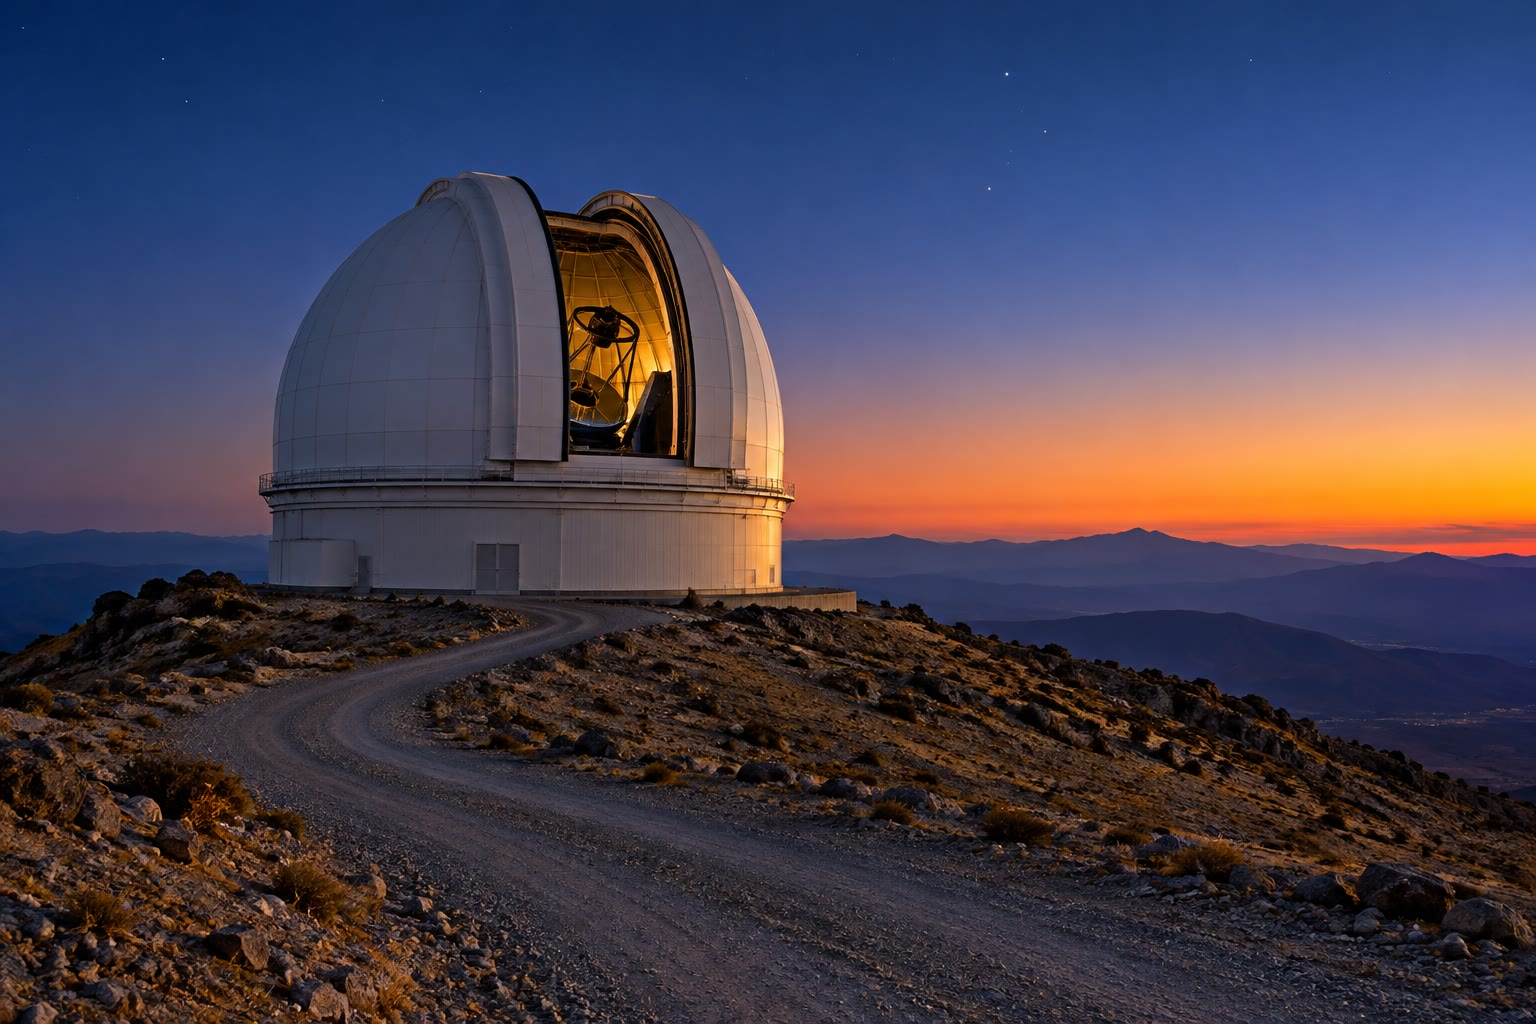
\includegraphics[width=0.55\linewidth]{images/book3/ai/b1-observatory-dusk.jpg}
\end{center}
\end{inthefield}

\section{फ़्लक्स और कांतियाँ}\label{sec:b1:observing-the-sky:magnitudes}

\begin{definition}[फ़्लक्स, दीप्ति]\label{def:b1:observing-the-sky:flux}
किसी स्रोत से प्राप्त \emph{फ़्लक्स}\index{फ़्लक्स (स्रोत का)} $F$ उसके विकिरण की वह शक्ति है जो उसकी दिशा
के लंबवत रखे इकाई क्षेत्रफल से वाट प्रति वर्ग मीटर में गुज़रती है; तरंगदैर्घ्यों के एक बैंड तक सीमित
होने पर वह उस बैंड का फ़्लक्स है। स्रोत की \emph{दीप्ति}\index{दीप्ति} $L$ वह कुल शक्ति है जो वह
विकिरित करता है, वाट में।
\end{definition}

\begin{proposition}[व्युत्क्रम-वर्ग नियम]\label{prop:b1:observing-the-sky:inverse-square}
\omterm{def:b1:observing-the-sky:flux}{दीप्ति} $L$ का एक स्रोत जो सभी दिशाओं में समान रूप से विकिरण करता है, और जो खाली आकाश में दूरी
$d$ से देखा जाए, यह \omterm{def:b1:observing-the-sky:flux}{फ़्लक्स} देता है
\[
  F = \frac{L}{4\pi d^2} .
\]
\end{proposition}

\begin{proof}
बिना अवशोषण की स्थिर अवस्था में, स्रोत पर केंद्रित किसी भी गोले से गुज़रती शक्ति ऊर्जा संरक्षण से
एक ही है, $L$। समरूपता से वह गोले के क्षेत्रफल $4\pi d^2$ पर समान रूप से फैलती है।
\end{proof}

\begin{example}
सूर्य की \omterm{def:b1:observing-the-sky:flux}{दीप्ति} \qty{3.828e26}{W} है। एक खगोलीय इकाई, \qty{1.496e11}{m} पर, उसका \omterm{def:b1:observing-the-sky:flux}{फ़्लक्स} है
$\num{3.828e26}/(4\pi\times
(\num{1.496e11})^2) = \qty{1361}{W.m^{-2}}$: वह सौर विकिरण-तीव्रता जो पृथ्वी को उसके वायुमंडल
के ऊपर मिलती है।
% ledger: sun:L, const:au, earth:TSI
\end{example}

\omterm{def:b1:observing-the-sky:flux}{फ़्लक्स} एक विशाल परास में फैले हैं, और खगोलविद उन्हें एक लघुगणकीय पैमाने पर तुलना करते हैं, जो
उन वर्गों से आया है जिनमें आँख से दिखने वाले तारे कभी छाँटे गए थे: सबसे चमकीले प्रथम कांति के,
सबसे मद्धम छठी कांति के।

\begin{definition}[दृश्य कांति, प्रकाशमितीय बैंड]\label{def:b1:observing-the-sky:magnitude}
\emph{प्रकाशमितीय बैंड}\index{प्रकाशमितीय बैंड} तरंगदैर्घ्यों का वह परास है जो एक मानक फ़िल्टर से चुना
जाता है और एक अक्षर से नामित होता है: U (पराबैंगनी), B (नीला), V (दृश्य), R (लाल), I (निकट अवरक्त),
और अवरक्त खिड़कियों में J, H, K। किसी बैंड में एक स्रोत की \emph{दृश्य कांति}\index{दृश्य कांति} $m$ उस
बैंड में उसके \omterm{def:b1:observing-the-sky:flux}{फ़्लक्स} $F$ से इस प्रकार परिभाषित है
\[
  m_1 - m_2 = -2.5\log_{10}\frac{F_1}{F_2} ,
\]
जिसमें शून्य-बिंदु मानक तारों से तय होता है, जो हर बैंड में वेगा तारे की कांति के लगभग बराबर है।
5 कांतियों का अंतर \omterm{def:b1:observing-the-sky:flux}{फ़्लक्स} में ठीक 100 गुने का अंतर है; एक कांति $100^{1/5} = 2.512$ गुना है।
उज्ज्वल स्रोतों की कांतियाँ छोटी, और संभवतः ऋणात्मक, होती हैं।
\end{definition}

मानक U, B, V, R और I फ़िल्टरों की मध्य तरंगदैर्घ्य \qty{358.5}{nm}, \qty{437.1}{nm}, \qty{547.8}{nm},
\qty{650.4}{nm} और \qty{802.0}{nm} हैं।
% ledger: baldry:bessell-pivot
V बैंड में सूर्य की \omterm{def:b1:observing-the-sky:magnitude}{दृश्य कांति} $-26.74$ है, रात के आकाश का सबसे उज्ज्वल तारा सिरियस $-1.46$, और
वेगा $0.03$ है। अतः सूर्य हमारे आकाश में सिरियस से $10^{0.4\times(26.74 - 1.46)} = \num{1.29e10}$ गुना
उज्ज्वल है; यह अभी नहीं बताता कि दोनों में से कौन वास्तव में अधिक चमकता है, जिसके लिए दूरियाँ चाहिए।
% ledger: nasa:sun-V, simbad:sirius, simbad:vega

\subsection*{लंबन और पारसेक}

जैसे-जैसे पृथ्वी सूर्य के चारों ओर घूमती है, एक निकट का तारा कहीं अधिक दूर की पृष्ठभूमि के तारों के
सापेक्ष खिसकता प्रतीत होता है, और एक वर्ष में एक छोटा दीर्घवृत्त खींचता है। वह आभासी गति तारों की
दूरियों का सबसे प्रत्यक्ष माप है: वह पृथ्वी की कक्षा को एक सर्वेक्षक के आधार-रेखा के रूप में प्रयोग करती है।

\begin{definition}[वार्षिक लंबन, पारसेक]\label{def:b1:observing-the-sky:parallax}
किसी तारे का \emph{वार्षिक लंबन}\index{वार्षिक लंबन} $p$ वह कोण है जो तारे पर पृथ्वी की कक्षा की
त्रिज्या, अर्थात् एक खगोलीय इकाई, दृष्टि-रेखा के लंबवत देखी जाने पर अंतरित करती है; यह उस वार्षिक
दीर्घवृत्त का अर्ध-दीर्घ अक्ष है जिसे तारा खींचता प्रतीत होता है। \emph{पारसेक}\index{पारसेक}
(\unit{\parsec}) वह दूरी है जिस पर एक खगोलीय इकाई एक चाप-सेकंड अंतरित करती है:
\[
  \qty{1}{\parsec} = \frac{\qty{1}{\au}}{\tan\ang{;;1}} = \qty{206265}{\au}
  = \qty{3.0857e16}{m} = \qty{3.2616}{\lightyear} .
\]
\end{definition}

चूँकि $p$ अत्यंत छोटा है, रेडियनों में $\tan p \approx p$ है, और दूरी तुरंत मिल जाती है:
\[
  d = \frac{\qty{1}{\au}}{\tan p} \quad\Longrightarrow\quad
  \frac{d}{\unit{\parsec}} = \frac{1}{p/\text{चाप-सेकंड}} .
\]
सिरियस का लंबन \ang{;;0.37921} है, अतः वह $1/0.37921 =
\qty{2.637}{\parsec}$, \qty{8.60}{\lightyear} पर है। सबसे निकटवर्ती तारों का भी लंबन एक चाप-सेकंड
से कम है, जो धुंधलेपन से छोटा है: लंबन तारे के प्रतिबिंब के केंद्र के खिसकने से मिलता है, जिसे
बहुत-से फ़ोटॉन प्रतिबिंब की चौड़ाई से कहीं अधिक सूक्ष्मता से स्थित करते हैं। इस अध्याय के अंत में
वर्णित एक अंतरिक्ष मिशन ने इसी ढंग से लगभग दो अरब वस्तुओं की स्थितियाँ मापी हैं।
% ledger: simbad:sirius, const:au, esa:gaia

\begin{omfigure}
\begin{tikzpicture}[font=\small]
\draw[black!50] (0,0) ellipse (2.0cm and 0.55cm);
\fill[orange!80!black] (0,0) circle (3pt) node[below=3pt] {सूर्य};
\fill[blue!70!black] (-2.0,0) circle (2pt) node[left, align=right] {छह महीने बाद\\ पृथ्वी};
\fill[blue!70!black] (2.0,0) circle (2pt) node[right] {पृथ्वी};
\fill (0,4.4) circle (1.6pt) node[above] {तारा};
\draw[omDef, thick] (0,0) -- node[right, pos=0.55] {$d$} (0,4.4);
\draw[omThm] (2.0,0) -- (0,4.4);
\draw[omThm, dashed] (-2.0,0) -- (0,4.4);
\draw[thick] (0,0) -- node[above] {\qty{1}{\au}} (2.0,0);
\draw[omThm] (0,3.75) arc[start angle=-90, end angle=-65.6, radius=0.65cm];
\node[omThm] at (0.17,3.38) {$p$};
\end{tikzpicture}

{\small \omterm{def:b1:observing-the-sky:parallax}{वार्षिक लंबन} (पैमाने पर नहीं): तारे से देखने पर पृथ्वी की कक्षा की त्रिज्या कोण $p$
अंतरित करती है। छह महीने के अंतर पर तारे की दिशा $2p$ से भिन्न होती है। निकटतम तारे का वास्तविक
कोण एक चाप-सेकंड से कम है।}
\end{omfigure}

\begin{definition}[निरपेक्ष कांति, दूरी-मापांक]\label{def:b1:observing-the-sky:absolute}
किसी बैंड में किसी तारे की \emph{निरपेक्ष कांति}\index{निरपेक्ष कांति} $M$ वह \omterm{def:b1:observing-the-sky:magnitude}{दृश्य कांति} है जो उसकी
\qty{10}{\parsec} की दूरी पर, खाली आकाश से देखे जाने पर, होती। अंतर $m - M$ उसका \emph{दूरी-मापांक}\index{दूरी-मापांक}
है।
\end{definition}

\begin{proposition}[दूरी-मापांक]\label{prop:b1:observing-the-sky:modulus}
खाली आकाश से देखे गए दूरी $d$ पर स्थित एक तारे के लिए
\[
  m - M = 5\log_{10}\frac{d}{\qty{10}{\parsec}} .
\]
यदि प्रकाश अपने मार्ग पर $A$ कांतियों के क्षीणन से मंद हो, तो
$m - M = 5\log_{10}(d/\qty{10}{\parsec}) + A$। किसी बैंड में दो तारों की दीप्तियों का अनुपात
$L_1/L_2 = 10^{0.4(M_2 - M_1)}$ है।
\end{proposition}

\begin{proof}
व्युत्क्रम-वर्ग नियम से $d$ पर \omterm{def:b1:observing-the-sky:flux}{फ़्लक्स} और \qty{10}{\parsec} पर \omterm{def:b1:observing-the-sky:flux}{फ़्लक्स} का अनुपात
$F(d)/F(\qty{10}{\parsec}) = (\qty{10}{\parsec}/d)^2$ है। कांतियों की परिभाषा $m - M = -2.5\log_{10}(\qty{10}{\parsec}/d)^2
= 5\log_{10}(d/\qty{10}{\parsec})$ देती है। क्षीणन \omterm{def:b1:observing-the-sky:flux}{फ़्लक्स} को $10^{-0.4A}$ से गुणा करता है, जो $A$ को $m$ में जोड़ता है।
समान दूरी \qty{10}{\parsec} पर \omterm{def:b1:observing-the-sky:flux}{फ़्लक्स} दीप्तियों के अनुपात में होते हैं, और $M_1 - M_2 = -2.5\log_{10}(L_1/L_2)$।
\end{proof}

सूर्य की \omterm{def:b1:observing-the-sky:absolute}{निरपेक्ष कांति} $M_\odot = 4.83$ और \omterm{def:b1:observing-the-sky:flux}{दीप्ति} \qty{3.828e26}{W} है। किसी तारे की V में \omterm{def:b1:observing-the-sky:absolute}{निरपेक्ष कांति} की
सूर्य की कांति से तुलना V बैंड में उसकी \omterm{def:b1:observing-the-sky:flux}{दीप्ति} सौर इकाइयों में देती है,
$L/L_\odot = 10^{0.4(4.83 - M)}$ --- एक \emph{V-बैंड} \omterm{def:b1:observing-the-sky:flux}{दीप्ति}, क्योंकि सूर्य से बहुत गर्म या ठंडा तारा अपनी
शक्ति का भिन्न भाग V बैंड के बाहर डालता है।
% ledger: sun:Mabs, sun:L

\subsection*{रंग}

\begin{definition}[वर्ण-सूचकांक]\label{def:b1:observing-the-sky:colour-index}
किसी तारे का \emph{वर्ण-सूचकांक}\index{वर्ण-सूचकांक} उसकी दो बैंडों की कांतियों का अंतर है, जो पहले
नीले बैंड की है; सबसे अधिक प्रयुक्त $B - V$ है। छोटा या ऋणात्मक $B - V$ नीला तारा दिखाता है, बड़ा
लाल तारा।
\end{definition}

\omterm{def:b1:observing-the-sky:colour-index}{वर्ण-सूचकांक} दूरी पर निर्भर नहीं करता, क्योंकि व्युत्क्रम-वर्ग नियम दोनों बैंडों को समान रूप से मंद
करता है; वह वर्णक्रम के आकार को मापता है, इसलिए तारे की सतह के तापमान को। तारा लगभग एक कृष्णिका
की तरह विकिरण करता है, जिसका वर्णक्रम $\lambda_\mathrm{max} = b/T$ पर शिखर बनाता है (वीन का नियम,
जिसमें $b = \qty{2.898e-3}{m.K}$, भौतिकी की पुस्तकों के दूसरे वर्ष से स्वीकृत)। नीचे की आकृति तीन
कृष्णिका वर्णक्रम दिखाती है: \qty{3500}{K} पर एक ठंडा पिंड निकट अवरक्त में शिखर बनाता है और V में
B की तुलना में अधिक \omterm{def:b1:observing-the-sky:flux}{फ़्लक्स} देता है; सूर्य का प्रभावी तापमान, \qty{5772}{K}, उसका शिखर
\qty{502}{nm} पर रखता है, B और V के बीच; \qty{10000}{K} पर एक पिंड पराबैंगनी में शिखर बनाता है और
B में V की तुलना में अधिक चमकीला है। तीनों वक्रों के लिए B और V विकिरणों का अनुपात तापमान के
साथ लगातार बढ़ता है, \num{0.46} से \num{0.97} और \num{1.53} तक, इसीलिए $B - V$ घटता है जब $T$ बढ़ता है।
% ledger: const:b, nasa:sun-Teff, baldry:bessell-pivot

\begin{omfigure}
\begin{tikzpicture}
\begin{axis}[omrecord, width=0.9\linewidth, height=5.8cm, xmin=200, xmax=1500,
  ymin=0, ymax=1.17, xtick={200,400,...,1400}, ytick={0,0.5,1},
  xlabel={तरंगदैर्घ्य (nm)},
  ylabel={$B_\lambda$ / अधिकतम}, tick label style={font=\scriptsize},
  label style={font=\small}, legend style={font=\scriptsize, at={(0.5,1.03)},
  anchor=south, draw=none, fill=none}, legend columns=3]
\addplot[red!75!black, line width=1.1pt] table[x=lam_nm, y=t3500] {figdata/out/bachelor-1-blackbody_bands-curves.dat};
\addplot[orange!90!black, line width=1.1pt] table[x=lam_nm, y=t5772] {figdata/out/bachelor-1-blackbody_bands-curves.dat};
\addplot[omDef, line width=1.1pt] table[x=lam_nm, y=t10000] {figdata/out/bachelor-1-blackbody_bands-curves.dat};
\legend{\qty{3500}{K}, \qty{5772}{K} (सूर्य), \qty{10000}{K}}
\draw[black!45, densely dashed] (axis cs:358.5,0) -- (axis cs:358.5,1.06);
\node[font=\scriptsize, above, inner sep=1pt] at (axis cs:358.5,1.06) {U};
\draw[black!45, densely dashed] (axis cs:437.1,0) -- (axis cs:437.1,1.06);
\node[font=\scriptsize, above, inner sep=1pt] at (axis cs:437.1,1.06) {B};
\draw[black!45, densely dashed] (axis cs:547.8,0) -- (axis cs:547.8,1.06);
\node[font=\scriptsize, above, inner sep=1pt] at (axis cs:547.8,1.06) {V};
\draw[black!45, densely dashed] (axis cs:650.4,0) -- (axis cs:650.4,1.06);
\node[font=\scriptsize, above, inner sep=1pt] at (axis cs:650.4,1.06) {R};
\draw[black!45, densely dashed] (axis cs:802.0,0) -- (axis cs:802.0,1.06);
\node[font=\scriptsize, above, inner sep=1pt] at (axis cs:802.0,1.06) {I};
\end{axis}
\end{tikzpicture}

{\small तीन तापमानों पर कृष्णिका वर्णक्रम, हर एक को अपने अधिकतम से भाग दिया गया, और U, B, V, R तथा I
फ़िल्टरों के मध्य तरंगदैर्घ्य (बिंदुरेखा)। तापमान बढ़ने पर शिखर छोटी तरंगदैर्घ्यों की ओर खिसकता है
(वीन का नियम): \qty{828}{nm}, \qty{502}{nm} और \qty{290}{nm}।}
% ledger: const:h, const:c, const:kB, const:b, nasa:sun-Teff, baldry:bessell-pivot
\end{omfigure}

तारों के रंगों का परास चार चमकीले तारे दिखाते हैं:
\begin{center}
\small
\begin{tabular}{lcccc}
\hline
तारा & $V$ & $B$ & $B - V$ & लंबन (\unit{mas}) \\
\hline
रीजेल & 0.13 & 0.10 & $-0.03$ & 3.78 \\
अल्टेयर & 0.76 & 0.98 & 0.22 & 194.95 \\
पोलारिस & 2.02 & 2.62 & 0.60 & 7.54 \\
बेटेल्जूज़ & 0.42 & 2.27 & 1.85 & 6.55 \\
\hline
\end{tabular}
\end{center}
% ledger: simbad:rigel, simbad:altair, simbad:polaris, simbad:betelgeuse
रीजेल नीला-श्वेत है और उसी तारामंडल का बेटेल्जूज़ नारंगी-लाल: एक ऐसा रंग-अंतर जो नंगी आँख को दिखता
है। उनके वर्णक्रमीय प्रकार, B8 और M1--M2, वर्णक्रम की भाषा में वही बात कहते हैं, जो पुस्तक 5
(स्नातक वर्ष 3) का विषय है।

\section{वर्णक्रमदर्शी}

प्रकाशमिति प्रकाश को कुछ चौड़े बैंडों में मापती है; वर्णक्रमदर्शी उसे एक वर्णक्रम में फैला देता है।
दूरबीन के फ़ोकस से आया प्रकाश एक संकरी दरार से गुज़रता है, एक संगमक द्वारा समांतर किया जाता है,
एक जाली (या प्रिज़्म) द्वारा विक्षेपित होता है, और एक कैमरे द्वारा संसूचक पर केंद्रित होता है, जहाँ
हर तरंगदैर्घ्य पिक्सेलों के एक अलग स्तंभ पर पड़ता है (नीचे की आकृति देखिए)। $N$ रेखाओं वाली जाली,
जो कोटि $k$ में प्रयुक्त होती है, दो तरंगदैर्घ्यों को, जो $\Delta\lambda$ दूर हैं, तब अलग करती है जब
$\lambda/\Delta\lambda \le kN$ हो; यह उसकी विभेदन-क्षमता है (भौतिकी की पुस्तकों के दूसरे वर्ष से स्मरण किया गया)।

\begin{omfigure}
\begin{tikzpicture}[font=\scriptsize, >=Stealth]
\draw[thick, fill=omSea!25] (0.15,0) ellipse (0.13 and 0.9);
\node[below] at (0.15,-0.95) {अभिदृश्यक};
\draw[omDef] (-1.3,0.75) -- (0.15,0.75) -- (2.4,0);
\draw[omDef] (-1.3,-0.75) -- (0.15,-0.75) -- (2.4,0);
\draw[omDef, ->] (-1.3,0) -- (-0.2,0);
\node[above] at (-0.8,0.75) {तारे का प्रकाश};
\draw[very thick] (2.4,-0.35) -- (2.4,-0.06); \draw[very thick] (2.4,0.06) -- (2.4,0.35);
\node[above] at (2.4,0.38) {दरार};
\draw[omDef] (2.4,0) -- (3.6,0.55); \draw[omDef] (2.4,0) -- (3.6,-0.55);
\draw[thick, fill=omSea!25] (3.6,0) ellipse (0.1 and 0.72); \node[below] at (3.6,-0.74) {संगमक};
\draw[omDef] (3.6,0.55) -- (4.9,0.55); \draw[omDef] (3.6,-0.55) -- (4.9,-0.55);
\draw[thick, pattern=north east lines] (4.85,-0.8) rectangle (5.0,0.8);
\node[below] at (4.92,-0.82) {जाली};
\draw[blue!70!black] (5.0,0.3) -- (6.4,0.95); \draw[red!70!black] (5.0,0.3) -- (6.4,-0.15);
\draw[blue!70!black] (5.0,-0.3) -- (6.4,0.35); \draw[red!70!black] (5.0,-0.3) -- (6.4,-0.75);
\draw[thick, fill=omSea!25] (6.4,0.1) ellipse (0.1 and 1.08); \node[below] at (6.4,-1.0) {कैमरा};
\draw[blue!70!black] (6.4,0.95) -- (7.6,0.55); \draw[blue!70!black] (6.4,0.35) -- (7.6,0.55);
\draw[red!70!black] (6.4,-0.15) -- (7.6,-0.45); \draw[red!70!black] (6.4,-0.75) -- (7.6,-0.45);
\fill[black!70] (7.6,-0.8) rectangle (7.75,0.9);
\node[right, align=left] at (7.8,0.05) {संसूचक:\\ हर स्तंभ पर एक तरंगदैर्घ्य};
\end{tikzpicture}

{\small एक दूरबीन और एक जाली वर्णक्रमदर्शी से प्रकाश का पथ (योजनाबद्ध, जिसमें दूरबीन का अभिदृश्यक और
प्रकाशिकी लेंसों के रूप में बनाए गए हैं, और दो तरंगदैर्घ्य): दरार तारे के प्रतिबिंब को अलग करती है,
संगमक किरण-पुंज को समांतर करता है, जाली उसे विक्षेपित करती है, और कैमरा हर तरंगदैर्घ्य को
संसूचक पर उसके अपने स्थान पर केंद्रित करता है।}
\end{omfigure}

वर्णक्रम तीन प्रकार की जानकारी रखता है। उसकी \emph{रेखाएँ}, जो तारे के वायुमंडल के
परमाणुओं और आयनों के सोखने पर काली और गर्म विरल गैस के उत्सर्जन पर चमकीली होती हैं, उपस्थित
रासायनिक तत्वों की पहचान कराती हैं। उसके सतत भाग का आकार, और अलग-अलग तापमानों पर बनी रेखाओं की
सापेक्ष प्रबलता, गैस का तापमान देती हैं। और रेखाओं का डॉप्लर विस्थापन दृष्टि-रेखा के अनुदिश वेग
देता है: विराम तरंगदैर्घ्य $\lambda$ वाली एक रेखा $\Delta\lambda = \lambda v_r/c$ से खिसकती है, रेडियल वेग
$v_r$ के लिए, जो $c$ से बहुत छोटा है। $v_r$ को \qty{1}{km.s^{-1}} तक मापने के लिए
लगभग $c/v_r = \num{300000}$ की विभेदन-क्षमता चाहिए, या एक मध्यम विभेदन-क्षमता और कई रेखाएँ
एक साथ मापना। तारों और आकाशगंगाओं की संरचना, संघटन और गतियाँ वर्णक्रम कैसे प्रकट करते हैं, वह
पुस्तक 5 (स्नातक वर्ष 3) का विषय है।

\section{अंतरिक्ष से प्रेक्षण}

वायुमंडल के ऊपर न कोई बंद खिड़कियाँ हैं, न क्षीणन, न \omterm{def:b1:observing-the-sky:seeing}{धुंधलापन}, और अवरक्त में गर्म हवा की कोई चमक।
अंतरिक्ष की दूरबीनें इसकी कीमत लागत से चुकाती हैं, उस सीमित द्रव्यमान और आकार से जो एक रॉकेट
प्रक्षेपित कर सकता है, और, उनमें से अधिकांश के लिए, मरम्मत की असंभवता से। वे वहाँ प्रयुक्त होती हैं
जहाँ ज़मीन मुक़ाबला नहीं कर सकती: गामा किरणों, X-किरणों और पराबैंगनी के लिए, जो कभी ज़मीन तक नहीं
पहुँचतीं; संकरी खिड़कियों से परे के अवरक्त के लिए; एक विस्तृत क्षेत्र पर विवर्तन-सीमा के प्रतिबिंबों
के लिए; और ऐसे मापनों के लिए, जैसे बहुत-से तारों के लंबन, जिनके लिए विक्षुब्ध वायु के बाहर एक स्थिर
उपकरण चाहिए।

\begin{dated}{2026}
% ledger: nasa:hubble-mirror, nasa:jwst-mirror, nasa:jwst-orbit, nasa:jwst-launch, nasa:jwst-range, esa:gaia
तीन अंतरिक्ष वेधशालाएँ इस परास को दिखाती हैं। हबल अंतरिक्ष दूरबीन, जो 1990 में प्रक्षेपित हुई, उसका
प्राथमिक दर्पण \qty{2.4}{m} आर-पार का है। जेम्स वेब अंतरिक्ष दूरबीन, जो 25 दिसंबर 2021 को प्रक्षेपित
हुई, उसका प्राथमिक दर्पण \qty{6.5}{m} आर-पार का है, जो 18 षट्कोणीय खंडों से बना है, और उसका
संग्रहण क्षेत्रफल \qty{25}{m^2} है; वह \qty{0.6}{\micro\metre} से \qty{28.5}{\micro\metre} तक काम
करती है और सूर्य की परिक्रमा पृथ्वी से \num{1.5} मिलियन किलोमीटर दूर, सूर्य से विपरीत ओर, दूसरे लाग्रांज
बिंदु L2 के पास करती है। गैया, जो 19 दिसंबर 2013 को उसी क्षेत्र में प्रक्षेपित हुई, उसने CCDs के एक
साझा फ़ोकल तल पर दो दूरबीनों से लगभग दो अरब वस्तुओं की स्थितियाँ और गतियाँ त्रि-विमीय में मानचित्रित
कीं; उसके प्रेक्षण पूरे हो चुके हैं, और उसकी सूचियाँ जारी की जा रही हैं।
\end{dated}

\begin{omfigure}
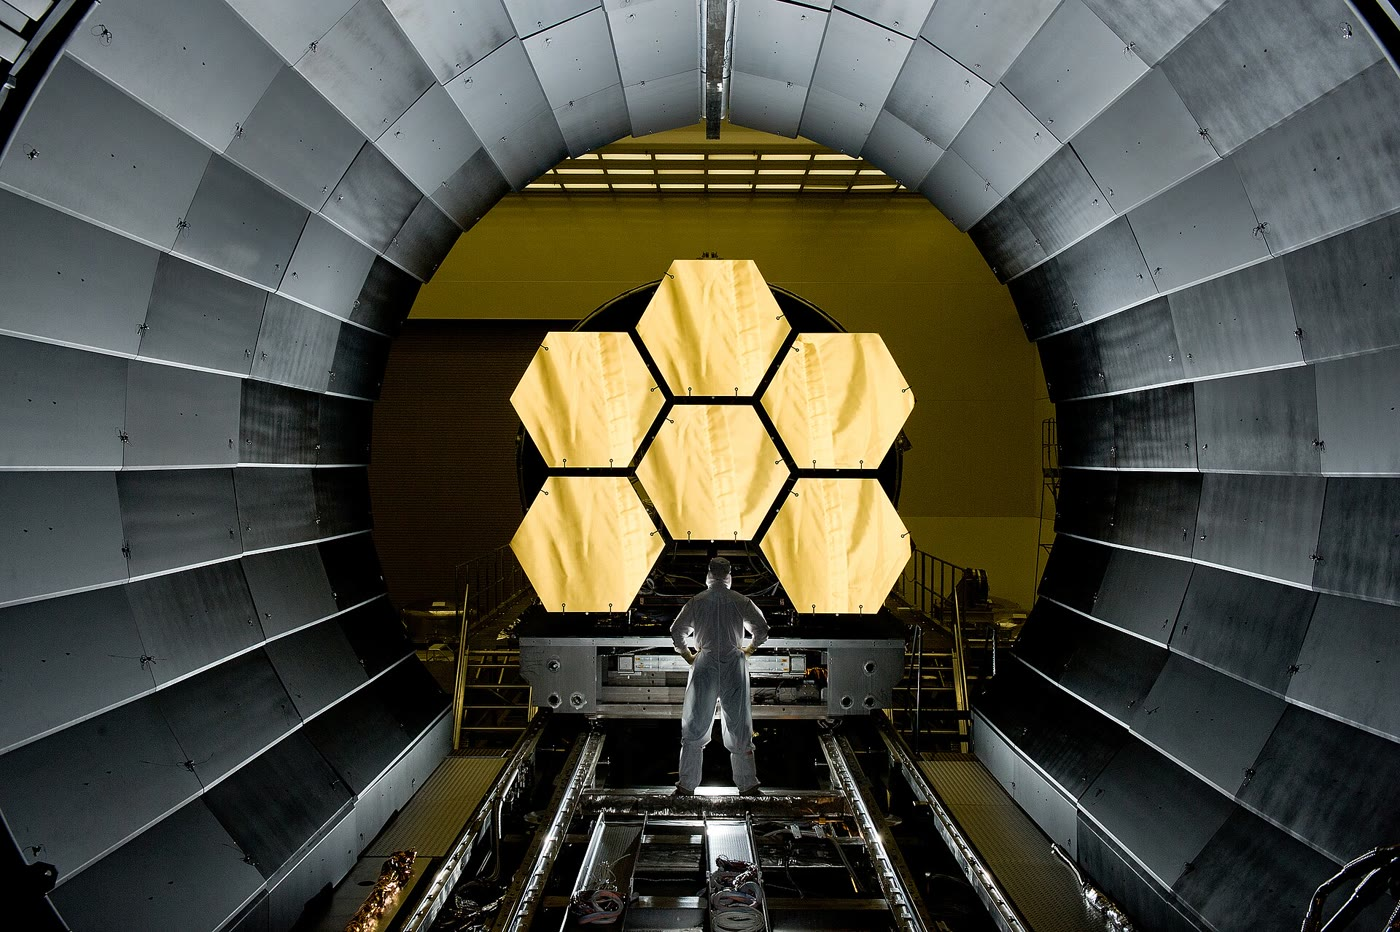
\includegraphics[width=0.78\linewidth]{images/book3/b1-jwst-mirror-segments.jpg}

{\small जेम्स वेब अंतरिक्ष दूरबीन के प्राथमिक दर्पण के 18 षट्कोणीय खंडों में से छह, जो 2011 में
शीत परीक्षण के लिए तैयार किए गए; अंतरिक्ष में खोले जाने पर 18 मिलकर \qty{6.5}{m} चौड़ा दर्पण
बनाते हैं। फ़ोटो: NASA/MSFC/डेविड हिगिनबॉथम, सार्वजनिक क्षेत्र।}
% ledger: commons:jwst-mirror, nasa:jwst-mirror
\end{omfigure}

\section{अभ्यास}

\begin{exercise}[$\star$]\label{exo:b1:observing-the-sky:1}
दो तारों के फ़्लक्सों का अनुपात क्या है जिनकी कांतियाँ 1.0 और 6.0 हैं? रीजेल ($V = 0.13$) और
पोलारिस ($V = 2.02$) का? आकाश में कौन अधिक चमकीला है?
\end{exercise}

\begin{exercise}[$\star$]\label{exo:b1:observing-the-sky:2}
अल्टेयर का लंबन \ang{;;0.19495} है। उसकी दूरी \omterm{def:b1:observing-the-sky:parallax}{पारसेक} में, खगोलीय इकाइयों में और प्रकाश-वर्षों में दीजिए।
\end{exercise}

\begin{exercise}[$\star$]\label{exo:b1:observing-the-sky:3}
\qty{2.4}{m} अंतरिक्ष दूरबीन की \qty{550}{nm} पर विवर्तन-सीमा चाप-सेकंड में परिकलित कीजिए, और उसकी
तुलना \ang{;;0.40} के धुंधलेपन से कीजिए। वही \qty{6.5}{m} दूरबीन के लिए \qty{2.0}{\micro\metre} पर कीजिए।
\end{exercise}

\begin{exercise}[$\star$]\label{exo:b1:observing-the-sky:4}
तालिका के चार चमकीले तारों में से रीजेल, अल्टेयर, पोलारिस और बेटेल्जूज़ को सबसे गर्म सतह से सबसे
ठंडी तक क्रम से रखिए। बहुत भिन्न दूरियों पर स्थित तारों के बीच \omterm{def:b1:observing-the-sky:colour-index}{वर्ण-सूचकांक} की तुलना क्यों की जा
सकती है?
\end{exercise}

\begin{exercise}[$\star\star$]\label{exo:b1:observing-the-sky:5}
एक तारे को एक ही रात में \ang{30} के खमध्य-दूरी कोण पर कांति 6.412 और \ang{60} पर 6.590 मापा
गया। समतल-समांतर वायुमंडल मानकर, दोनों वायु-राशियाँ, क्षीणन गुणांक और वायुमंडल के ऊपर तारे की
कांति परिकलित कीजिए।
\end{exercise}

\begin{exercise}[$\star\star$]\label{exo:b1:observing-the-sky:6}
एक तारा \qty{10}{s} के अनावरण में 400 प्रकाश-इलेक्ट्रॉन देता है, और अकेले तारे का फ़ोटॉन शोर प्रधान
है। \omterm{def:b1:observing-the-sky:detector}{सिग्नल-से-शोर अनुपात} क्या है? 100 का SNR पाने के लिए कितनी देर तक अनावरण करना होगा? कांति को
\num{0.01} तक मापने के लिए?
\end{exercise}

\begin{exercise}[$\star\star$]\label{exo:b1:observing-the-sky:7}
रीजेल का $V = 0.13$ है और लंबन \ang{;;0.00378} है। हमारे और उसके बीच क्षीणन की उपेक्षा करते हुए, उसकी
दूरी, उसकी \omterm{def:b1:observing-the-sky:absolute}{निरपेक्ष कांति} और V बैंड में सौर इकाइयों में उसकी \omterm{def:b1:observing-the-sky:flux}{दीप्ति} परिकलित कीजिए ($M_\odot = 4.83$)।
\end{exercise}

\begin{exercise}[$\star\star$]\label{exo:b1:observing-the-sky:8}
\qty{2.4}{m} के एक वृत्ताकार दर्पण (उसकी केंद्रीय रुकावट की उपेक्षा कीजिए) और वेब दूरबीन
(\qty{25}{m^2}) के संग्रहण क्षेत्रफलों की तुलना कीजिए। वेब दूरबीन उतने ही फ़ोटॉन एकत्र करने में
कितने कम समय का अनावरण लेती है? \qty{6.5}{m} आर-पार की एक पूरी चकती का कितना भाग उसका संग्रहण
क्षेत्रफल दर्शाता है, और वह एक से कम क्यों है?
\end{exercise}

\begin{exercise}[$\star\star$]\label{exo:b1:observing-the-sky:9}
(क) सूर्य की \omterm{def:b1:observing-the-sky:flux}{दीप्ति} \qty{3.828e26}{W} से, \qty{10}{\parsec} पर उसका \omterm{def:b1:observing-the-sky:flux}{फ़्लक्स} परिकलित कीजिए। (ख) सूर्य की
दृश्य और निरपेक्ष कांतियाँ $-26.74$ और $4.83$ हैं। \omterm{def:b1:observing-the-sky:absolute}{दूरी-मापांक} से सूर्य-पृथ्वी दूरी खगोलीय इकाइयों
में पुनः प्राप्त कीजिए।
\end{exercise}

\begin{exercise}[$\star\star\star$]\label{exo:b1:observing-the-sky:10}
\cref{prop:b1:observing-the-sky:bouguer} से दिखाइए कि $k =
2.5\log_{10}e\;\tau_0$ है। क्षीणन रेखा की रात के लिए ($k =
\num{0.160}$), \omterm{def:b1:spherical-astronomy:celestial-sphere}{खमध्य} प्रकाशीय गहराई $\tau_0$ और \omterm{def:b1:spherical-astronomy:celestial-sphere}{खमध्य} पर तथा $X = 2.31$ पर दूरबीन तक पहुँचने वाले
प्रकाश का भाग परिकलित कीजिए। \ang{85} की खमध्य-दूरी पर समतल-समांतर वायुमंडल \omterm{def:b1:observing-the-sky:extinction}{वायु-राशि} के लिए क्या
अनुमान देगा, और उस मान पर भरोसा क्यों नहीं करना चाहिए?
\end{exercise}

\begin{exercise}[$\star\star\star$]\label{exo:b1:observing-the-sky:11}
एक मंद आकाशगंगा दूरबीन में प्रति सेकंड $R = 50$ प्रकाश-इलेक्ट्रॉन देती है, और जब \omterm{def:b1:observing-the-sky:seeing}{धुंधलापन}
\ang{;;0.80} हो तब उसके प्रतिबिंब के क्षेत्र का आकाश प्रति सेकंड $B = \num{2000}$ देता है। पठन-शोर
नगण्य है। (क) 10 के SNR के लिए कितनी देर अनावरण करना होगा? (ख) प्रतिबिंब का आकाश धुंधलेपन की चकती
के क्षेत्रफल के साथ बढ़ता है। \ang{;;0.40} के धुंधलेपन के लिए दोहराइए। (ग) दिखाइए कि आकाश से बहुत
मंद स्रोत के लिए, दिए गए SNR के लिए आवश्यक अनावरण-काल $\theta^2/D^2$ के अनुपात में बदलता है, जहाँ
$\theta$ \omterm{def:b1:observing-the-sky:seeing}{धुंधलापन} है और $D$ दूरबीन का व्यास।
\end{exercise}

\begin{exercise}[$\star\star\star$]\label{exo:b1:observing-the-sky:12}
प्रति मिलीमीटर 1200 रेखाओं वाली एक जाली \qty{100}{mm} पर प्रकाशित है और पहली कोटि में प्रयुक्त
होती है। (क) उसकी विभेदन-क्षमता क्या है, और \qty{550}{nm} पर सबसे छोटा पृथक्करणीय तरंगदैर्घ्य-अंतर?
(ख) वह अंतर किस रेडियल वेग के अनुरूप है? (ग) पृथ्वी \qty{29.78}{km.s^{-1}} पर सूर्य की परिक्रमा
करती है। यह गति \qty{550}{nm} की रेखा को कितना खिसका सकती है, और वह कितने विभेदन तत्वों के बराबर
है? इसलिए एक प्रेक्षक को, जो किसी तारे का वेग माप रहा है, क्या करना चाहिए?
% ledger: earth:vorb
\end{exercise}

\section{समस्या: सिरियस का प्रकाश तौलना}

\begin{problem}[{सप्ताहांत समस्या --- सिरियस कितना दूर है, वह कितना चमकीला दिखता है और कितने फ़ोटॉन
भेजता है, और वह कितने सूर्यों से अधिक चमकता है}]
\label{pb:b1:observing-the-sky:1}
% ledger: simbad:sirius, simbad:vega, simbad:sirius-b, nasa:sun-V, sun:Mabs, const:au
% numbers computed in the scratch calculator calc/ch02.py from the rounded data
सिरियस, रात के आकाश का सबसे चमकीला तारा, एक मद्धम साथी रखता है, श्वेत बौना सिरियस~B। आँकड़े लीजिए:
\begin{center}
\small
\begin{tabular}{lcc}
\hline
वस्तु & $V$ & लंबन \\
\hline
सिरियस & $-1.46$ & \ang{;;0.37921} \\
सिरियस B & $8.44$ & --- \\
वेगा & $0.03$ & \ang{;;0.13023} \\
सूर्य & $-26.74$ & --- \\
\hline
\end{tabular}
\end{center}
V में $M_\odot = 4.83$, $\qty{1}{\parsec} = \qty{206265}{\au} =
\qty{3.0857e16}{m} = \qty{3.2616}{\lightyear}$ के साथ, और वेधशाला पर प्रति \omterm{def:b1:observing-the-sky:extinction}{वायु-राशि} क्षीणन गुणांक
$k = 0.15$।

\medskip
\noindent\textbf{भाग I --- सिरियस कितना दूर है?}
\begin{enumerate}
  \item सिरियस की दूरी \omterm{def:b1:observing-the-sky:parallax}{पारसेक} में परिकलित कीजिए।
  \item उसे खगोलीय इकाइयों और मीटरों में व्यक्त कीजिए।
  \item उसे प्रकाश-वर्षों में व्यक्त कीजिए। आज रात हम जो प्रकाश देखते हैं, वह सिरियस से कितने समय पहले चला था?
  \item एक वर्ष में सिरियस की दिशा कुल कितने कोण तक एक ओर से दूसरी ओर झूलती है? उसकी तुलना \ang{;;0.40} के धुंधलेपन से कीजिए। झूलना अब भी धुंधलेपन के एक छोटे भाग तक क्यों मापा जा सकता है?
  \item यदि लंबन \ang{;;0.001} गलत होता, तो दूरी किस भाग से गलत होती, और कितने प्रकाश-वर्ष से?
\end{enumerate}

\medskip
\noindent\textbf{भाग II --- वह कितना चमकीला दिखता है?}
\begin{enumerate}[resume]
  \item V में सिरियस और वेगा के फ़्लक्सों का अनुपात परिकलित कीजिए।
  \item सूर्य और सिरियस के फ़्लक्सों का अनुपात परिकलित कीजिए।
  \item सिरियस और सिरियस~B के फ़्लक्सों का अनुपात परिकलित कीजिए।
  \item पैरानाल वेधशाला से सिरियस \ang{82.09} के \omterm{def:b1:spherical-astronomy:horizontal}{उन्नतांश} पर याम्योत्तर पार करता है (\cref{ch:b1:spherical-astronomy})। उस क्षण पर मापी गई \omterm{def:b1:observing-the-sky:extinction}{वायु-राशि}, क्षीणन और कांति परिकलित कीजिए।
  \item \ang{30} के \omterm{def:b1:spherical-astronomy:horizontal}{उन्नतांश} पर दोहराइए। मार्ग में प्रकाश का कितना भाग खो जाता है?
  \item सिरियस के उगने के ठीक बाद उसे मापने वाले प्रेक्षक को सूत्र $X = \sec z$ क्यों भ्रमित करेगा?
\end{enumerate}

\medskip
\noindent\textbf{भाग III --- फ़ोटॉन गिनना।}
\qty{1}{m} की दूरबीन पर एक कैमरा, क्षीणन के लिए सुधार के बाद, प्रति सेकंड $\num{3.0e4}$ प्रकाश-इलेक्ट्रॉन
दर्ज करता है, और यह एक ऐसे तारे से है जिसकी कांति $V = 10.0$ है। हर पिक्सेल अधिकतम
$\num{1.0e5}$ इलेक्ट्रॉन (उसका पूर्ण कूप) रख सकता है।
\begin{enumerate}[resume]
  \item इस कैमरे पर सिरियस~B से प्रति सेकंड कितने प्रकाश-इलेक्ट्रॉन दर्ज होते हैं?
  \item कितना अनावरण सिरियस~B को, केवल तारे के फ़ोटॉन शोर के साथ, 1000 का SNR देगा? तब उसकी कांति पर त्रुटि क्या होगी?
  \item इस कैमरे पर सिरियस से प्रति सेकंड कितने प्रकाश-इलेक्ट्रॉन दर्ज होते हैं?
  \item यदि सिरियस का \qty{20}{\percent} प्रकाश उसके सबसे चमकीले पिक्सेल में पड़े, तो वह पिक्सेल भरने में कितना समय लेता है?
  \item कैमरे पर सिरियस के मंद पंख सिरियस~B के स्थान पर प्रति पिक्सेल सिरियस के प्रकाश का $10^{-4}$ जमा करते हैं, और सिरियस~B का सबसे चमकीला पिक्सेल अपने ही प्रकाश का \qty{20}{\percent} एकत्र करता है। उस पिक्सेल में दोनों दरों की तुलना कीजिए।
  \item वह सबसे लंबा अनावरण क्या है जो उस पिक्सेल को संतृप्त नहीं करता? \qty{0.5}{s} के अनावरण में उस पिक्सेल में सिरियस~B का SNR परिकलित कीजिए, दोनों स्रोतों का फ़ोटॉन शोर गिनते हुए। क्या सिरियस~B पहचाना जा सकता है, और उसे कठिन क्या बनाता है?
\end{enumerate}

\medskip
\noindent\textbf{भाग IV --- कितने सूर्य?}
\begin{enumerate}[resume]
  \item सिरियस का \omterm{def:b1:observing-the-sky:absolute}{दूरी-मापांक} परिकलित कीजिए।
  \item दो दशमलव तक सिरियस की V में \omterm{def:b1:observing-the-sky:absolute}{निरपेक्ष कांति} निकालिए।
  \item सिरियस और वेगा की दूरी और \omterm{def:b1:observing-the-sky:absolute}{निरपेक्ष कांति} परिकलित कीजिए।
  \item सिरियस और वेगा में से कौन-सा V में आंतरिक रूप से अधिक दीप्त है, और किस गुणक से?
  \item सिरियस की दूरी से देखे गए सूर्य की \omterm{def:b1:observing-the-sky:magnitude}{दृश्य कांति} क्या होगी? अँधेरी रात में नंगी आँख को दिखने वाली सबसे मंद कांति 6.0 मानते हुए, क्या वह दिखेगा?
  \item सिरियस किस दूरी तक नंगी आँख को दिखता रहेगा?
  \item सिरियस की V-बैंड \omterm{def:b1:observing-the-sky:flux}{दीप्ति} सौर इकाइयों में परिकलित कीजिए: सिरियस कितने सूर्यों से अधिक चमकता है?
\end{enumerate}
\end{problem}
